\documentclass{minimal}

\usepackage{pgf}
\usepackage{tikz}
\usetikzlibrary{arrows,automata}
\usetikzlibrary{positioning}

\begin{document}

\begin{tikzpicture}[->,>=stealth']

	\node[initial,state,accepting,node distance=3cm]	(q4) [below of=q1]	{$q4$};
	\node[state,node distance=2cm]	(q0) [left of=q1]  {$q_0$};
	\node[state]	(q1)							 {$q_1$};
	\node[state,node distance=2cm]	(q2) [right of=q1]  {$q_2$};
	\node[state,node distance=2cm]	(q3) [right of=q2]  {$q_3$};
	
	\path[->]	(q4) edge [loop below] node[auto] {$a$} (q4);
	\path[->]	(q4) edge [bend left=20] node[auto] {$\neg a$} (q0);
	\path[->]	(q0) edge [bend left=20] node[auto] {$a$} (q4);
	\path[->]	(q0) edge [] node[auto] {$\neg a$} (q1);
	\path[->]	(q1) edge [] node[auto] {$a$} (q4);
	\path[->]	(q1) edge [] node[auto] {$\neg a$} (q2);
	\path[->]	(q2) edge [] node[auto] {$a$} (q4);
	\path[->]	(q2) edge [loop above] node[auto] {$\neg a \land \neg b$} (q2);
	\path[->]	(q2) edge [bend right=45] node[above] {$\neg a \land b$} (q0);
	\path[->]	(q2) edge [] node[above] {$c$} (q3);
	\path[->]	(q3) edge [bend left=20] node[auto] {$always$} (q4);
\end{tikzpicture}

\begin{itemize}
	\item \textbf{$a$:} reset=true
	\item \textbf{$b$:} Alle Pixel im aktuellen Kernel analysiert=true
	\item \textbf{$c$:} Alle Pixel des Bildes analysiert=true	
\end{itemize}



\begin{itemize}
	\item \textbf{$q0$:} Erster Warte-Zustand zwischen dem Anlegen der Speicheradresse am Block RAM und dem Auslesen der Daten
	\item \textbf{$q1$:} Erster Warte-Zustand zwischen dem Anlegen der Speicheradresse am Block RAM und dem Auslesen der Daten
	\item \textbf{$q2$:} Analysieren der ausgelesenen Daten
	\item \textbf{$q3$:} Überschreiben der gefundenen ROIs von einem Bufffer in das Ausgaberegister	
	\item \textbf{$q4$:} Reset-Zustand, der die Variablen auf einen Anfangszustand zurück setzt	
\end{itemize}

\textbf{Beschreibung der Pixel-Analyse:}\\
Durch das Anlegen einer Adresse an den Block-RAM, wird das Auslesen initialisiert und nach 2 Clock-Takten können die Daten der entsprechenden Adresse, am Ausgang des Speichers,  abgegriffen werden.
Pro Speichereinheit enthält der RAM 255 Bit Daten, die sich aus 32 Pixeln mit je 8 Bit Intensitätswert, zusammensetzen. Für diesen Vorgang sind die Zustände $q0$ und $q1$ zuständig.\\
Die Analyse wird pixelweise durchgeführt. Überschreitet die Intensität des Pixels einen definierten Grenzwert, wird er als Kandidat für einen Spot in Betracht gezogen. Im Anschluss wird überprüft, ob der Pixel bereits in einer ROI enthalten ist, sollte dies nicht der Fall sein, werden basierend auf den Parametern ROI\_width und ROI\_height, 2 Punkte ermittelt, die ein Rechteck um den Spot aufspannen. Die beiden Punkte entsprechen der linken oberen und der rechten unteren Ecke des Rechteckes und werden entsprechend angepasst, damit sie definitiv im Bild liegen.

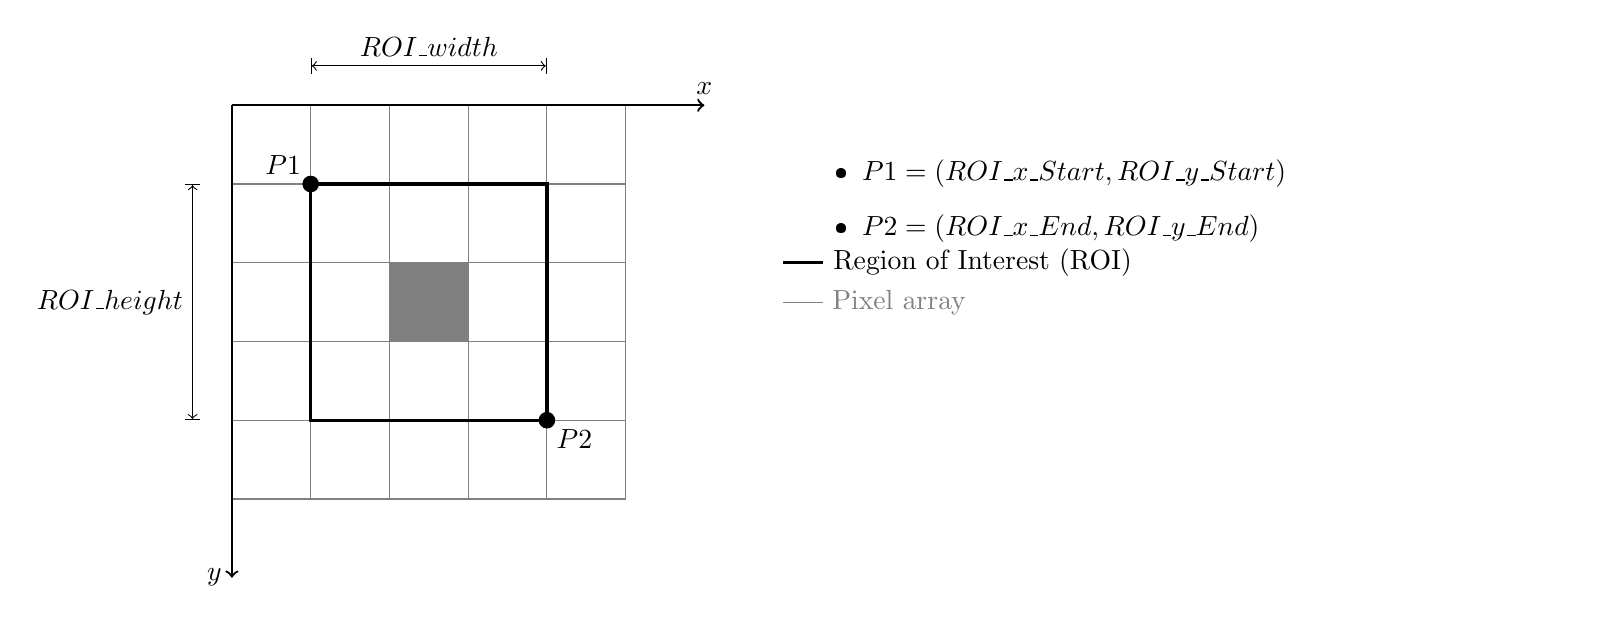
\begin{tikzpicture}
	\draw[gray]  (0,0) grid (5,5);
	\draw[very thick] (1,1) rectangle (4,4);
	\fill[gray] (2,2) rectangle (3,3);
	
	\draw[|<->|] (-0.5,1) -- node [left]{$ROI\_height$} (-0.5,4);
	\draw[|<->|] (1,5.5) -- node [above]{$ROI\_width$} (4,5.5);
	
	\fill (1,4) circle (3pt) node [above left]{$P1$};
	\fill (4,1) circle (3pt) node [below right]{$P2$};
	
	\draw[thick,->] (0,5)--(0,-1) node [left] {$y$};	
	\draw[thick,->] (0,5)--(6,5)node [above] {$x$};
	
	
	\node[right,text width=10cm] at (7,4) 
	{\begin{itemize}
		 \item $P1=(ROI\_x\_Start,ROI\_y\_Start)$
		 \item $P2=(ROI\_x\_End,ROI\_y\_End)$		
	\end{itemize}};
	
	\draw[very thick] (7,3)--(7.5,3) node [right]{Region of Interest (ROI)};
	\draw[gray] (7,2.5)--(7.5,2.5) node [right]{Pixel array};
\end{tikzpicture}


\end{document}